\subsection{The link-analysis algorithm}\label{sec:background:linkanalysis}

The \textit{link-analysis} algorithm is an adaption of a web page ranking algorithm HITS \cite{kleinberg1999authoritative} to the recommendation domain \cite{huang2004link, huang2007comparison}.

The original algorithm distinguish between two types of web pages:

\begin{enumerate}
    \item \textit{Authoritative} pages which contain definite high quality information
    \item \textit{Hub} pages basically are lists of links to the authoritative pages
\end{enumerate}

The authoritative score of a page is proportional to the hub scores linking to it. Similarly the hub score of a page is proportional to the authoritative scores of the pages it is linking to. These definitions are mutually reinforcing, good hub pages have links to many authoritative pages and good authoritative pages have links from many hubs.

Adaptation to the recommendation domain is achieved by introducing the \textit{item representativeness} score $\IR$ and the \textit{user representativeness} score $\UR$. The difference between the recommendation domain and the web page ranking domain is that in the recommendation domain the aim is to produce personal recommendations where as in the web page domain generally popular pages are sought after.

The \textit{item representativeness} score $\IR(i, u)$ can be seen as a measure of the item $i$'s level of interest with respect to user $u$, or in other words $i$'s authority of $u$'s interests in $i$. This is an analogy to the authoritative page score. Intuitively if it is a high score then the item $i$ can be recommended to user $u$.

The \textit{user representativeness} score $\UR(u, \hat{u})$ measures how well $u$ as a hub for $\hat{u}$ associates with items of interests to $\hat{u}$. This is analogous to the hub page score. Intuitively it is a measure for how similar the users $u$ and $\hat{u}$ are to each other.

A direct definition of the item and user representativeness scores is as follows where $A$ is the interaction matrix:

\begin{equation}
    \IR = A^T * \UR
\end{equation}

\begin{equation}
    \UR = A * \IR
\end{equation}

There are two inherent problems with these definitions. The first is if a user has interactions with all items then that user will have the highest user representativeness $\UR$ for all users, even though such a user provides little information. The second problem is that $\IR$ and $\UR$ will converge to matrices with identical columns. This leads to item representativeness scores $\IR(i, u)$ which are independent of the user $u$ chosen and depend only on the item $i$.  \cite{huang2004link, huang2007comparison}

To address these problems the user representativeness score is redefined \cite{huang2007comparison} as

\begin{equation}
    \UR = B * \IR + \UR_0
\end{equation}

Where $B$ is the normalization of the users $A$ with respect to the total number of items the user has interacted with

\begin{equation}
    B_{u, i} = \frac{ A_{u, i} }{ \left(\sum_{i} A_{u, i}\right)^\gamma }
\end{equation}

The effect of introducing $B$ is that a user $u$ with more item interactions than another user $\hat{u}$, to get a high user representativeness score $\UR(u, \hat{u})$ the user $u$ needs to have overlapping purchases with $\hat{u}$. The parameter $\gamma$ controls the extent to which a user is penalized for making many purchases.

$\UR_0$ is defined as a diagonal matrix with $\eta$ on the diagonal. In other words $\UR_0 = \eta * I_M$ where $I_M$ is an $M\,x\,M$ identity matrix and $M$ is the number of users. It is included to maintain the high representativeness score for the target users themselves, which prevents $\IR$ and $\UR$ to converge to identical columns.

This also necessitates a normalization step of $\UR$ to keep the values on a consistent level, otherwise numerical problems could occur when the values keep growing.

In summary the \textit{link-analysis} algorithm follow these steps:

\begin{enumerate}
    \item Construct the interaction matrix $A$ and the associating matrix $B$.

    \item Set $\UR_0 = \eta * I_M$.
    \item At each iteration $t = 1, \ldots, t_{max}$ perform:

        \begin{enumerate}
            \item $\IR_t = A^T * \UR_{t- 1}$
            \item $\UR_t = B * \IR_t$
            \item Normalize $\UR_t$ so each column adds up to 1
            \item $\UR_t = \UR_t + \UR_0$
        \end{enumerate}

        Repeat until convergence.

    \item The predicted matrix is given by $P = \IR^T$.

\end{enumerate}

\newpage
\subsubsection{Runtime example}

This is a runtime example for \textit{link-analysis} using a simple interaction matrix \eqref{eq:exA}, corresponding to the interaction graph \figureref{fig:ex_graph}.

\begin{equation}\label{eq:exA}
  A = \kbordermatrix{
    &    i_1 & i_2 & i_3 & i_4 \\
    u_1 & 0   & 1   & 0   & 1  \\
    u_2 & 0   & 1   & 1   & 1  \\
    u_3 & 1   & 0   & 1   & 0
  }
\end{equation}

\begin{figure}[h!]
    \centering
    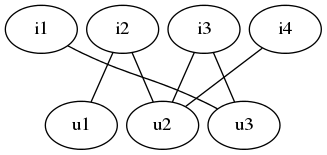
\includegraphics[width=0.3\linewidth]{fig/example_run/item_user_graph.png}
    \caption{A graph representing the interaction history between each user and item, describing the interaction matrix in \eqref{eq:exA}.}
    \label{fig:ex_graph}
\end{figure}

The following example uses $\gamma = 0.9$ and $\eta = 1$.

\[
  B = \kbordermatrix{
    &    i_1 & i_2 & i_3 & i_4 \\
    u_1 & 0         & 0.5359    & 0         & 0.5359  \\
    u_2 & 0         & 0.3720    & 0.3720    & 0.3720  \\
    u_3 & 0.5359    & 0         & 0.5359    & 0
  },
\;
  \UR_0 = \kbordermatrix{
    &    u_1 & u_2 & u_3 \\
    u_1 & 1   & 0  & 0  \\
    u_2 & 0   & 1  & 0  \\
    u_3 & 0   & 0  & 1
  }
\]

During the iterations the rows of $\IR$ will be representing each item and each column will be representing each user, this is the reverse of the interaction matrix $A$. The example therefore presents the transpose of $\IR$, $\IR^T$.

\[
    \IR^T_1 = \left(A^T * \UR_0\right)^T 
    = \kbordermatrix{
        &    i_1 & i_2 & i_3 & i_4 \\
        u_1 &     0 & 1 & 0 & 1 \\
        u_2 &     0 & 1 & 1 & 1 \\
        u_3 &     1 & 0 & 1 & 0
    }
\]
\[
\UR_1
= norm\left(B * \IR_1\right) + \UR_0 
    = \kbordermatrix{
      &    u_1 & u_2 & u_3 \\
      u_1 &  1.5902 & 0.4098 & 0 \\
      u_2 &  0.3935 & 1.4098 & 0.1967 \\
      u_3 &  0      & 0.2577 & 1.7423
    }
\]

\FloatBarrier

\begin{figure}[h!]
    \centering
    \begin{subfigure}[h!]{0.3\textwidth}
        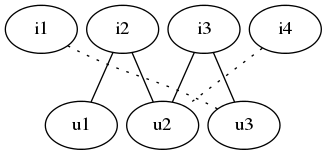
\includegraphics[width=\textwidth]{fig/example_run/item_user_ir1.png}
        \caption{$\IR_1$}
    \end{subfigure}
    ~
    \begin{subfigure}[h!]{0.15\textwidth}
        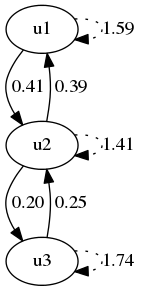
\includegraphics[width=\textwidth]{fig/example_run/user_user_ur1.png}
        \caption{$\UR_1$}
        \label{fig:link:ur1}
    \end{subfigure}
    \caption{Visual representation of the first iteration. The full lines in $\UR_1$ (b) represents new connections, which come from the new connections in $\IR_1$ (a) also represented by full lines.}
    \label{fig:link:it1}
\end{figure}

The first iteration does not alter the item representativeness matrix. In the user representativeness matrix links between users are made through one shared item.  As seen in \figureref{fig:link:it1} a connection is made between $u_1$ and $u_2$, through $i_2$ and a connection between $u_2$ and $u_3$ through $i_3$.

\FloatBarrier

\[
    \IR^T_2 = \left(A^T * \UR_1\right)^T 
    = \kbordermatrix{
        &    i_1 & i_2 & i_3 & i_4 \\
        u_1 &      0 &  2.0000 &  0.4098 &  2.0000 \\
        u_2 & 0.1967 &  1.8033 &  1.6065 &  1.8033 \\
        u_3 & 1.7423 &  0.2577 &  2.0000 &  0.2577
    }
\]
\[
    \UR_2
    = norm\left(B * \IR_2\right) + \UR_0 
    = \kbordermatrix{
      &    u_1 & u_2 & u_3 \\
      u_1 &   1.5354 &  0.4098 &  0.0548 \\
      u_2 &   0.3994 &  1.4008 &  0.1997 \\
      u_3 &   0.0858 &  0.2909 &  1.6233
    }
\]

\FloatBarrier

\begin{figure}[h!]
    \centering
    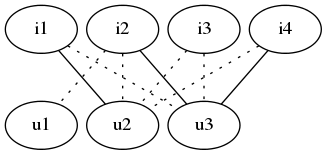
\includegraphics[width=0.3\textwidth]{fig/example_run/item_user_ir2.png}
    \caption{Visual representation of $\IR_2$. The full lines represents new connections.}
    \label{fig:link:ir2}
\end{figure}

\FloatBarrier

New connections in $\IR_2$ are made by using item connections from related users from $\UR_1$. In \figureref{fig:link:ir2} new connections for $u_3$ are made to $i_2$ and $i_4$ because $u_2$ is now representing $u_3$ in \figureref{fig:link:ur1}, and $u_2$ has connections with $i_2$ and $i_4$.

\newpage % Layout things!
\[
    \IR^T_3 = \left(A^T * \UR_2\right)^T 
    = \kbordermatrix{
        &    i_1 & i_2 & i_3 & i_4 \\
        u_1 & 0.0548 &  1.9452 &  0.4646 &  1.9452 \\
        u_2 & 0.1997 &  1.8003 &  1.6006 &  1.8003 \\
        u_3 & 1.6233 &  0.3767 &  1.9142 &  0.3767
    }
\]
\[
    \UR_3
    = norm\left(B * \IR_3\right) + \UR_0 
    = \kbordermatrix{
        &    u_1 & u_2 & u_3 \\
        u_1 & 1.5234 &  0.4067 &  0.0699 \\
        u_2 & 0.3995 &  1.4007 &  0.1998 \\
        u_3 & 0.1226 &  0.3015 &  1.5759
    }
\]

After transposing $\IR_3$ and removing the items users already have interacted with in $A$, the prediction matrix $P$ becomes

\[
  P = \kbordermatrix{
    &    i_1 & i_2 & i_3 & i_4 \\
    u_1 &     0.0548 &  0 &  \mathbf{0.4646} &  0 \\
    u_2 &     \mathbf{0.1997} &  0 &  0 &  0 \\
    u_3 &     0 &  \mathbf{0.3767} &  0 &  \mathbf{0.3767}
  }
\]

\Figureref{fig:ex_graph_link_rec} is a visualization of $P$ displaying the single most recommended item for each user.

\begin{figure}[h!]
    \centering
    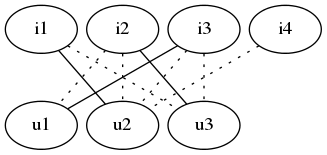
\includegraphics[width=0.3\linewidth]{fig/example_run/item_user_graph_link_rec.png}
    \caption{A graph representing the most recommended item for each user. The dotted lines represent the interaction history.}
    \label{fig:ex_graph_link_rec}
\end{figure}

\FloatBarrier

